% PROGETTO BASI DI DATI 2015 , MERLINO GIUSEPPE is CEO and VIOLETTO MIKI is SGUATTERO
%
% stato della relazione :
%
% abstract da rileggere e forse modificare
% analisi dei requisiti da cambiare un bel pò, aspetterei di farlo dopo aver fatto la progettazione concettuale, almeno l'inizio
% progettazione concettuale rimodellata, da rileggiere da capo, molte frasi da migliorare che sicuramente ho scritto cazzate
% immagini da controllare e posizionare meglio, tipo la grandezza 

%
\documentclass[a4paper,twoside]{article}

\usepackage[margin=3cm]{geometry}
\usepackage[utf8]{inputenc}
\usepackage[main=italian, english]{babel}
\usepackage{graphicx}
\usepackage{rotating}
\usepackage{verbatim}
\usepackage{listings}
\usepackage[colorlinks=true,linkcolor=black,urlcolor=blue]{hyperref} % ancore delle varie sezioni sul menu
\usepackage{float}

%\graphicspath{Immagini/} %non va ... bho

\author{Giuseppe Merlino,Miki Violetto}
\title{Relazione progetto BiciRent}
\date{\today}

\begin{document}
\maketitle

\newpage
\tableofcontents
\newpage
\listoffigures
\newpage

%  link utili
%  http://www.goodbikepadova.it/Default.aspx : GoodBike, dove prendiamo spunto per il progetto
%  www.lucidchart.com : programma per fare i grafici dei schemi concettuale e logico
%

\section{Abstract}
BiciRent è un servizio di bike sharing ispirato a Goodbike presente qui a Padova.\newline
Permette grazie ad una tessera personale di noleggiare in qualsiasi momento una delle bici presenti in apposite stazioni collocate in diverse aree della città ed utilizzarla per muoversi, lasciandola poi in un'altra stazione dove sia presente un posto libero.\newline
La tessera ha validità specifica a seconda del piano che si sottoscrive, e sono previsti sconti per studenti e turisti.\newline
Le biciclette noleggiabili sono di due tipi, quella classica munita di un passeggino oppure quella a pedalata assistita.\newline
Le stazioni sono presenti in molti aree della città e sono munite di sicure automatiche antifurto. Saranno sempre presenti biciclette da noleggiare e posti per lasciare la bici noleggiata grazie ad un servizio di trasporto e le biciclette rotte verranno sostituite da nuove.\newline
Il servizio tende ad essere automatizzato e permette all'abbonato di controllare facilmente se in una data stazione siano presenti biciclette o ci siano posti vuoti per depositare la bici noleggiata. Può segnalare la presenza di guasti delle biciclette.\newline
Si prospettano circa 1700 noleggi giornalieri e una media di 200 richieste d'intervento al giorno (mancanza di bici e rotture); inoltre viene richiesta la composizione dei posti di ogni singola stazione (presenza biciclette, tipi disponibili e posti liberi) almeno 3000 volte ogni giorno, ma con punte di quasi 900 richieste in una singola mezz'ora (ad esempio nelle ore di punta).

\section{Descrizione testuale dei requisiti e operazioni tipiche}
%Alias analisi dei requisiti XD
Si vuole realizzare una base di dati e una semplice applicazione web che contenga e gestisca le informazioni relative al bike sharing, simulando inoltre le operazioni che è possibile eseguire tramite la colonnina.

\subsection{Descrizione testuale}
Sono necessarie le informazioni personali degli utenti per permettergli di registrarsi e comprare una tessera; saranno quindi obbligatori nome e cognome, la data e il luogo di nascita, le informazioni sulla residenza (via, numero civico, città, C.A.P.) e un indirizzo email, l'utente può inserire il suo numero telefonico (campo facoltativo) per ricevere ulteriori informazioni.\newline
Per poter poi usufruire di convenzioni rilasciate solo a studenti, sarà necessario il codice di matricola in caso di universitari o l'id della carta Io Studio, e le agevolazioni verranno fornite solo per abbonamenti da mensili in su.\newline
Nel caso di turisti non è necessaria nessuna informazione aggiuntiva, ma l'agevolazione verrà fornita solo ai piani giornalieri, weekend o settimanali.\newline
La tessera personale, che verrà utilizzata per identificare l'utente in tutte le operazioni che effettuerà, avrà una validità data dal piano associato ad essa (giornaliera, per un singolo fine settimana, oppure essere collegata ad un abbonamento di varie taglie: settimanale, mensile, trimestrale, semestrale o annuale) e non potrà mai rimanere senza piano.\newline 
Un utente con piano ancora valido (attivo) potrà usufruire di tutti i servizi, mentre un utente con una tessera non più valida (piano scaduto) potrà solo comprare un nuovo piano ad un prezzo prefissato, da cui verrà tolto il 15\% per i turisti che usufruiscono dell'agevolazione e del 10\% per gli studenti.\newline
Le biciclette, identificate da un id univoco, possono essere a pedalata assistita (elettriche) oppure con un seggiolino (la maggior parte), mentre in base al loro stato sono suddivise tra biciclette in servizio (ferme alla colonnina o noleggiate), in deposito o biciclette danneggiate; lo stato di una bicicletta non sempre corrisponde alla propria posizione, infatti una bici danneggiata può  essere presente in magazzino o presso una colonnina.\newline
La  colonnina, identificata da un codice numerico e dalla stazione di cui fa parte, presenta uno stato: libera, occupata (a seconda della presenza o meno di una bicicletta) o danneggiata se la colonnina è guasta.\newline
Una stazione é formata da più colonnine e si utilizza anche in questo caso un id per l'identificazione; avrà un attributo contenente l'indirizzo di ubicazione, per facilitare la ricerca nelle mappe. L'utente interagirà con la stazione per conoscere gli stati delle varie colonnine (ma non si interesserà del singolo stato di ogni colonnina).

\subsection{Operazioni tipiche}
Operazioni tipiche eseguite dall'utente :
\paragraph{Prelievo di una bicicletta} Il noleggio interessa una bici in servizio che sta attualmente occupando una colonnina. Prendendo la bici in comodato, lo stato della colonnina cambia in "libera" e ciò genera un noleggio di tipo pendente, dove vengono memorizzati i dati della bicicletta noleggiata, la colonnina di prelievo e l'orario di prelievo. Un utente può avere un singolo noleggio attivo alla volta.
\paragraph{Deposito di una bicicletta} Il deposito interessa sempre una bicicletta in servizio, l'operazione modifica un noleggio pendente in uno di tipo terminato, salvando quindi la colonnina in cui viene depositata la bici e l'orario di deposito; questo porta la colonnina, che prima era libera, nello stato di occupata.
\paragraph{Controllo dello stato di una stazione} Controlla lo stato di ogni singola colonnina della stazione, e ritorna quanti spazi liberi e quante biciclette per tipo sono presenti.
\paragraph{Segnalazione mancanza di biciclette o spazi vuoti} Una segnalazione di tipo mancanza viene chiamata dall'utente tramite il sito oppure il numero telefonico su una data stazione e comporterà uno o più trasporti per assolvere la segnalazione.
\paragraph{Segnalazione di rottura} Una segnalazione di rottura viene chiamata dall'utente da una singola colonnina o dal sito e comporterà un ordine di manutenzione che potrà interessare la colonnina o la bicicletta.
\par Operazioni tipiche non effettuate dall'utente :
\paragraph{Trasporto di una bicicletta} Il trasporto può avvenire perché segnalato da un utente oppure per esigenze interne, e comporta il movimento di una bicicletta in tre modi diversi: tra due colonnine di diverse stazioni, dal magazzino ad una colonnina oppure da una colonnina al magazzino. Il trasporto di una bicicletta cambia sicuramente lo stato della colonnina interessata, e forse cambia anche lo stato della bicicletta.
\paragraph{Manutenzione di una colonnina o di una bicicletta} La manutenzione può avviene a seguito di una segnalazione oppure può essere richiesta dall'azienda e prevede un controllo della bicicletta o della colonnina, che verrà riassunto in una descrizione dei danni presenti che sono stati riparati, e dall'orario di fine manutenzione. Si nota che la manutenzione di una bicicletta interessa la colonninna su cui è stata presente, e che per semplicità ed efficienza viene sempre controllata sia la colonnina che la bicicletta se presente.Un'operazione di matunenzione comporterà per la colonnina e la bicicletta un cambio di stato (erano daneggiate, ora non lo sono più).
\par Operazioni dell'area amministrativa :
\paragraph{resoconto dei lavori di manutenzione} E' visibile dall'area amministrativa un resoconto dei lavori di manutenzione alle biciclette e alle colonnine dello scorso mese. Con riportati le date e gli orari.
\paragraph{storico di una bicicletta} Può venire richiesto dall'area amministrativa le manutenzioni di una bicicletta, come gli utenti che l'hanno noleggiata e il tempo in cui è stata noleggiata.
\paragraph{lista dei mezzi danneggiati} Può venire richiesta una lista delle biciclette danneggiate, con la stazione e l'area in cui sono presenti.

\subsection{Nuovi requisiti}
Dopo un'esposizione e un ragionamento sulle operazioni da eseguire, si possono delineare delle prime modifiche da effettuare alla descrizione testuale :
\paragraph{Operazioni di diverso spessore} Si nota che operazioni quali noleggio-deposito, segnalazione, trasporto e manutentione non sono semplici operazioni unitarie, ma coinvolgono molteplici operazioni.
\paragraph{modifica dello stato della bicicletta} Lo stato di una bicicletta non può venire rappresentato solo con in uso, in magazzino o danneggiata; Si decide di utilizzare 2 caratteristiche : lo stato della bicicletta (operativa o danneggiata) e la sua posizione (magazzino o in uso); Questo comporta un miglior rappresentazione dello stato della bicicletta.
\paragraph{Realtà su due livelli} Si nota che si potrebbe dividere la realtà d rappresentare in due parti: una parte si occupa dello stato attuale del sistema, quindi di dove attualmente sono le bici, della presenza di collonnine vuote o piene, etc mentre un'altra si occupa dello storico di queste informazioni, quindi dei noleggi terminati, dei trasorti effettuati, delle manutenzioni, etc.

\section{Progettazione concettuale}
%top-down , bottom-up, inside-out , misto

Per la modellazione concettuale si decide di partire dall'operazione principale del sistema che stiamo modellando, il noleggio.

\subsection{Noleggio}
Il noleggio è formato da due distinte operazioni, un prelievo che inizia il noleggio, e un deposito che lo termina; il deposito distingue inoltre il noleggio pendente, cioè non ancora terminato, con il noleggio terminato che fa parte di una specie di storico dei noleggi.
\begin{figure}[H]
 \centering
  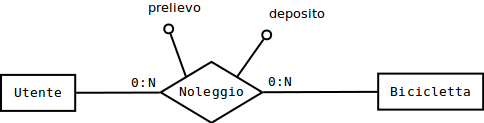
\includegraphics[width=0.5\textwidth]{Immagini-Grafici/Concettuale01.png}
\caption{Relazione noleggio}
\end{figure}
In un primo momento modelliamo il noleggio come una relazione che lega utenti e biciclette, ma questa relazione non ci soddisfa molto quindi decidiamo di eseguire subito il raffinamento e passare direttamente ad una entità noleggio.
\begin{figure}[H]
 \centering
  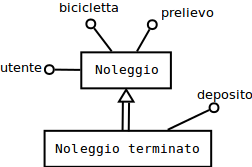
\includegraphics[width=0.5\textwidth]{Immagini-Grafici/Concettuale02.png}
\caption{Entità noleggio}
\end{figure}

\subsection{Utente}
Le informazioni personali dell'utente vengono rappresentate con l'entità Utente; Studente e Turista sono specializzazioni parziali esclusive.
\begin{figure}[H]
 \centering
  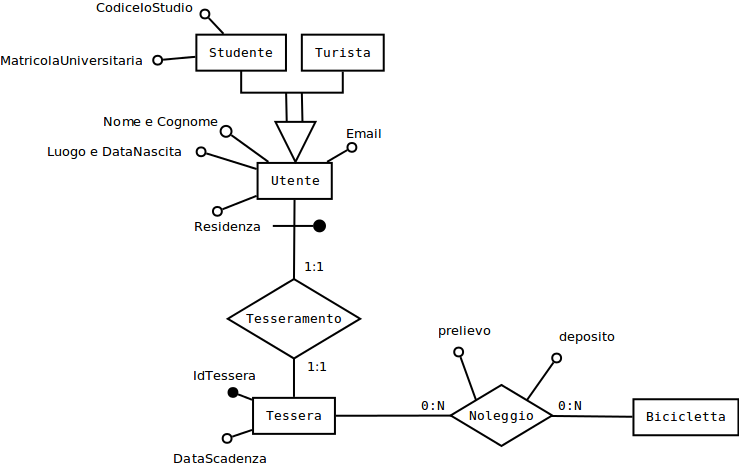
\includegraphics[width=0.5\textwidth]{Immagini-Grafici/Concettuale03.png}
\caption{Reificazione di utente}
\end{figure}

\subsection{Tessera}
La tessera personale dell'utente lo rappresenta in tutte le operazioni che esegue nel sito.
\begin{figure}[H]
 \centering
  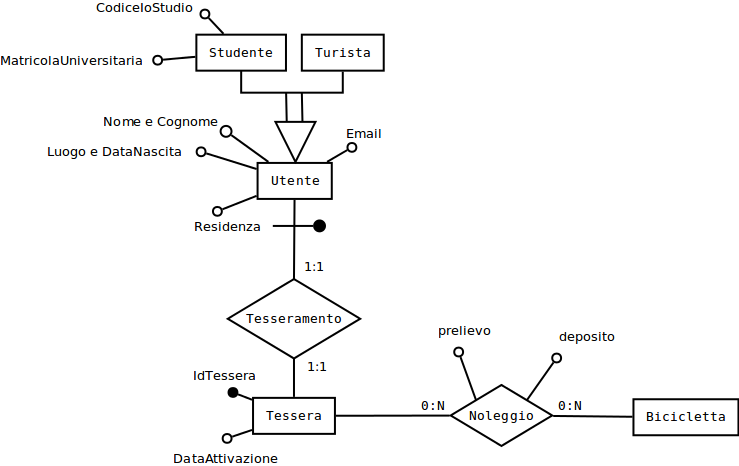
\includegraphics[width=0.5\textwidth]{Immagini-Grafici/Concettuale04.png}
\caption{Reificazione di tessera}
\end{figure}

\subsection{Piano}
Gli abbonamenti delle tessere corrispondondo alla sottoscrizione di un piano che ha un costo e identifica la validità della tessera.
\begin{figure}[H]
 \centering
  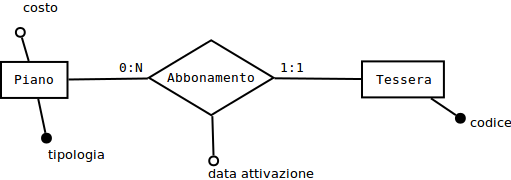
\includegraphics[width=0.5\textwidth]{Immagini-Grafici/Concettuale05.png}
\caption{Reificazione di piano}
\end{figure}

\subsection{Bicicletta}
Le biciclette possono essere in servizio, ferme o danneggiate (specializzazioni globali esclusive)
\begin{figure}[H]
 \centering
  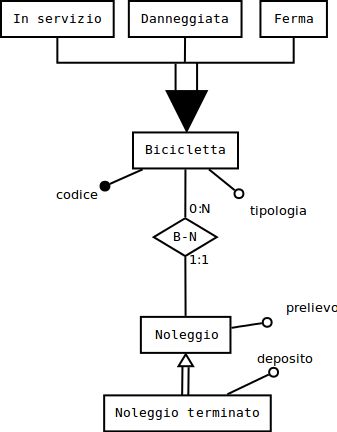
\includegraphics[width=0.5\textwidth]{Immagini-Grafici/Concettuale06.png}
\caption{Reificazione di bicicletta}
\end{figure}

\subsection{Operazione}
Sia prelievo che depositano presentano la data, l'orario e la colonnina interessata dall'operazione, quindi si introduce l'entità Operazione.
\begin{figure}[H]
 \centering
  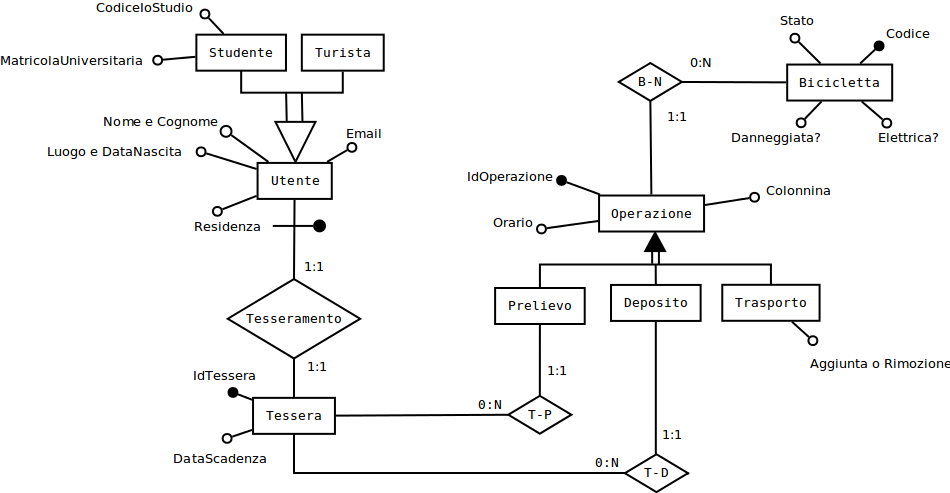
\includegraphics[width=0.5\textwidth]{Immagini-Grafici/Concettuale07.png}
\caption{Reificazione di prelievo e deposito}
\end{figure}

\subsection{Colonnina}
Le operazioni prelevano o depositano le biciclette su una colonnina, e un'operazione di deposito su una colonnina la fa diventare occupata, cioè vi è una bicicletta presente.
\begin{figure}[H]
 \centering
  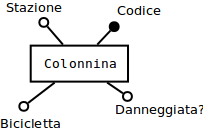
\includegraphics[width=0.5\textwidth]{Immagini-Grafici/Concettuale08.png}
\caption{Reificazione di colonnina}
\end{figure}

\subsection{Stazione}
Le colonnine sono racconte tra lono in stazioni.
\begin{figure}[H]
 \centering
  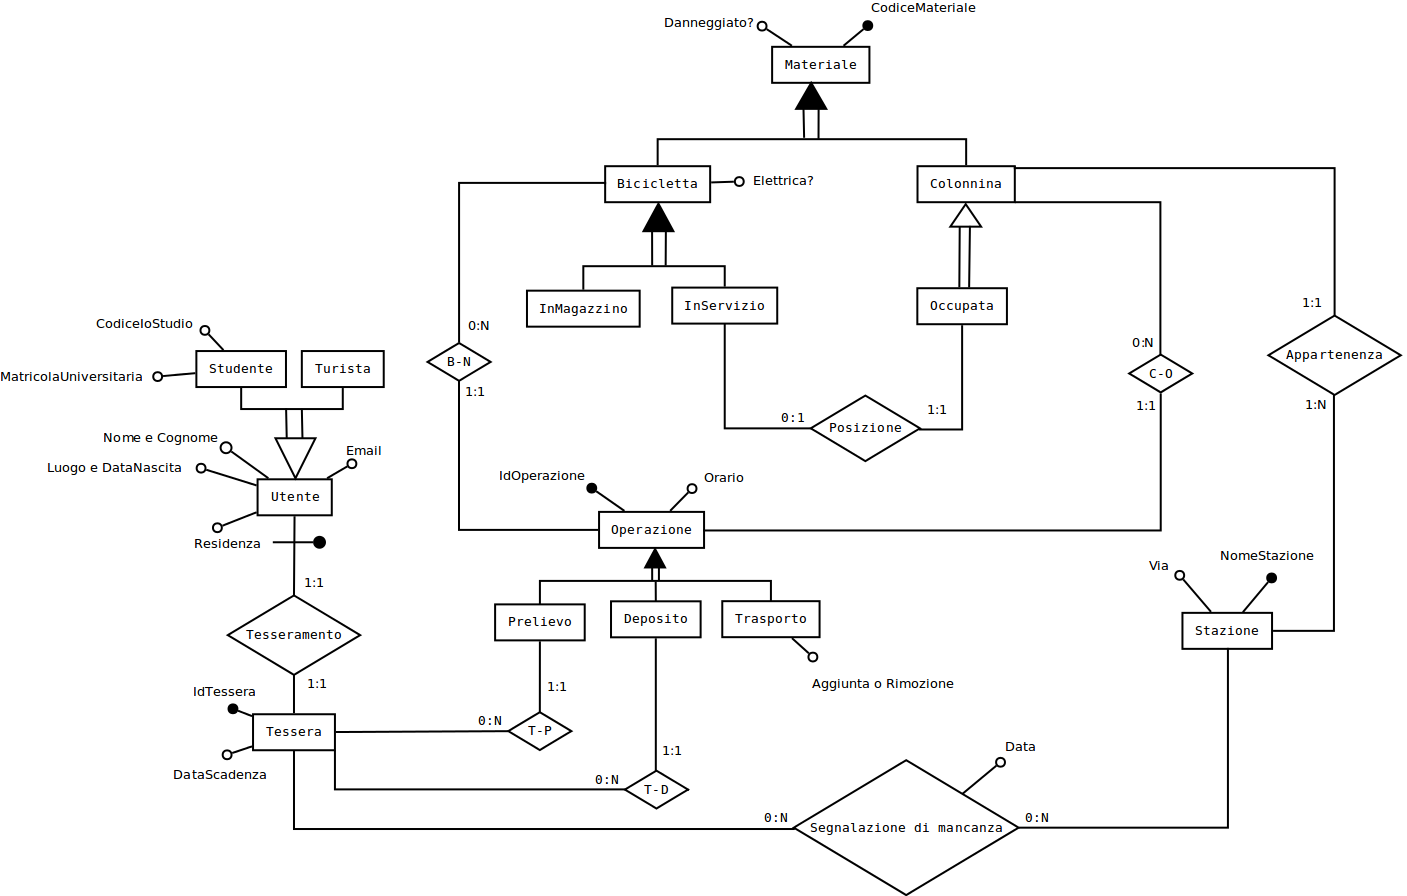
\includegraphics[width=0.5\textwidth]{Immagini-Grafici/Concettuale09.png}
\caption{Reificazione di stazione}
\end{figure}

\subsection{Segnalazione di mancanza}
Un utente può segnalare la mancanza di spazi liberi o di biciclette in una stazione
\begin{figure}[H]
 \centering
  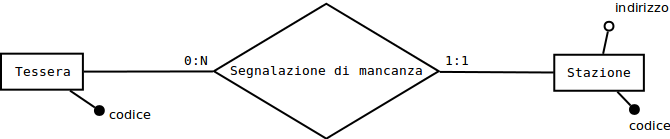
\includegraphics[width=0.5\textwidth]{Immagini-Grafici/Concettuale10.png}
\caption{Aggiunta delle segnalazioni di mancanza}
\end{figure}

\subsection{Segnalazione di rottura}
Un utente può segnalare una rottura, indicando una colonnina rotta o la bicicletta presente (se presente)
\begin{figure}[H]
 \centering
  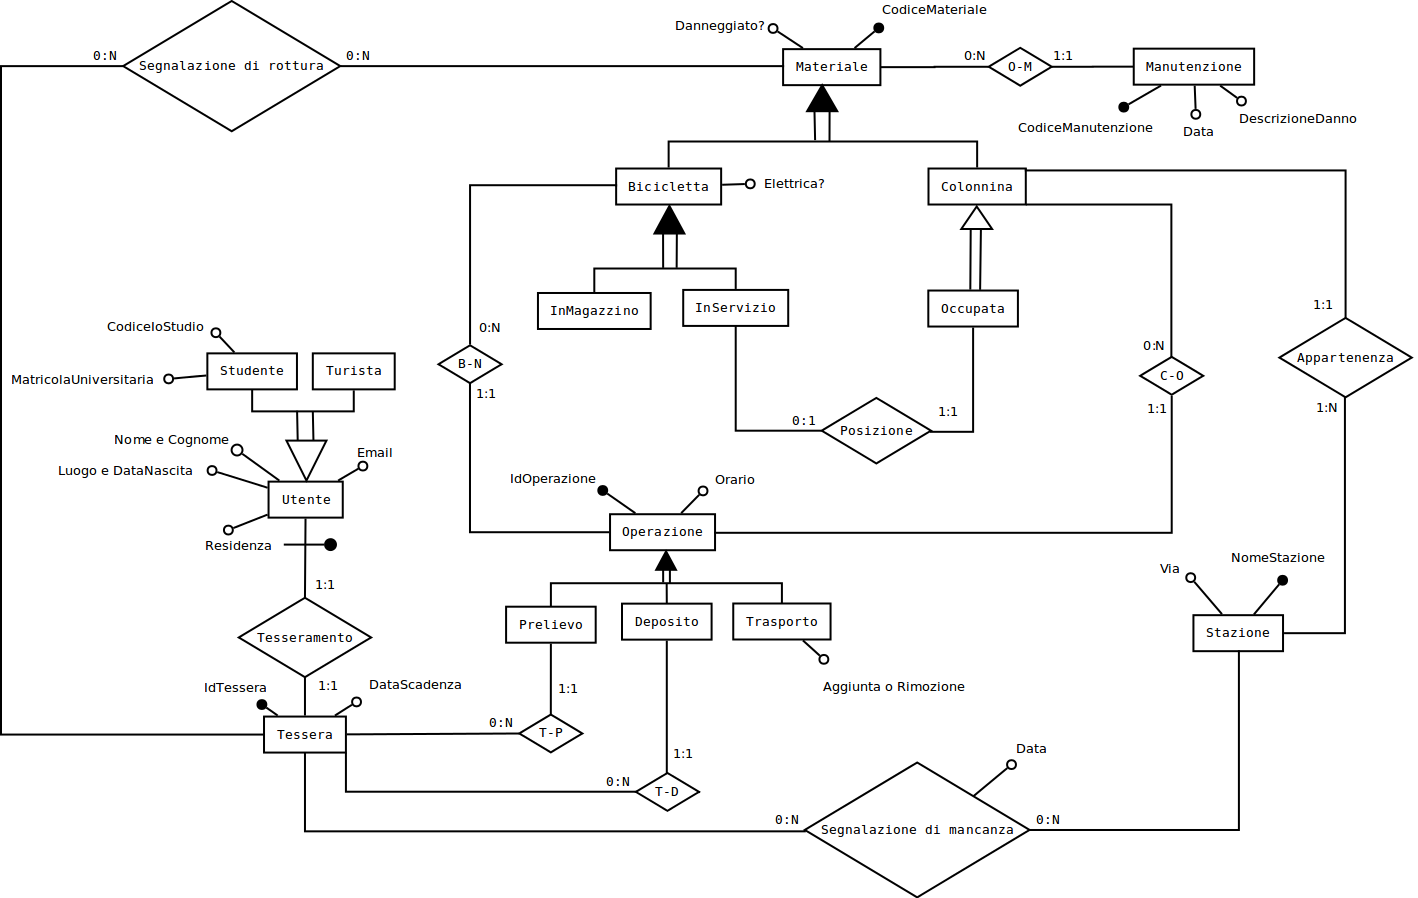
\includegraphics[width=0.5\textwidth]{Immagini-Grafici/Concettuale11.png}
\caption{Aggiunta delle segnalazioni di rottura}
\end{figure}

\subsection{Manutenzione}
Una colonnina oppure una bicicletta possono subire un intervento di manutenzione (per togliere lo stato danneggiato
\begin{figure}[H]
 \centering
  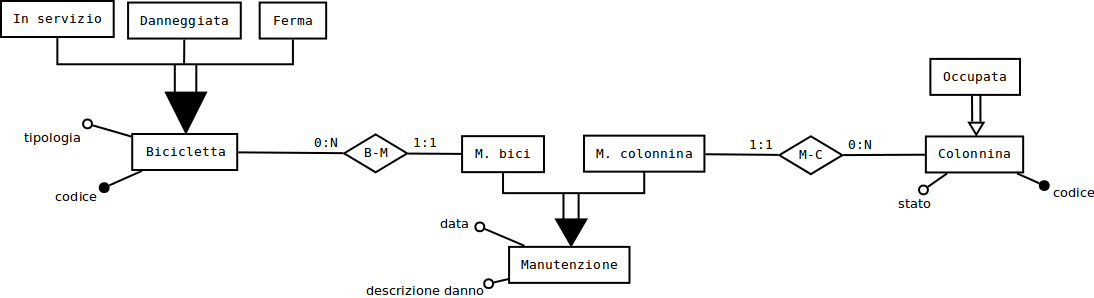
\includegraphics[width=0.5\textwidth]{Immagini-Grafici/Concettuale12.png}
\caption{Aggiunta delle manutenzioni}
\end{figure}

\subsection{Trasporto}
Per rappresentare i trasporti mi accorgo che avrei già un modello simile: le operazioni di prelievo e deposito; i trasporti differiscono dalla presenza di queste due operazioni(solo prelievo,solo deposito o entrambe).
\begin{figure}[H]
 \centering
  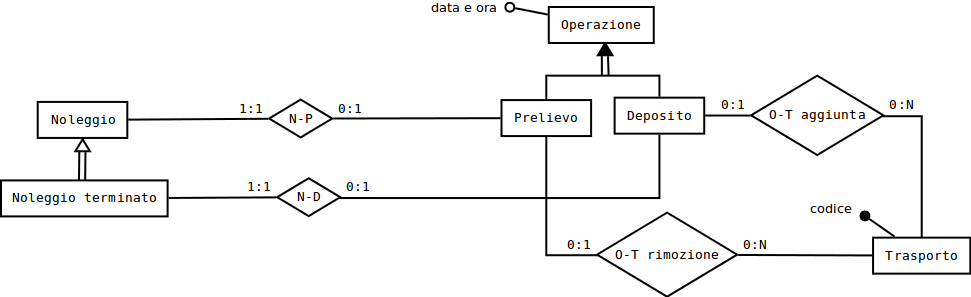
\includegraphics[width=0.5\textwidth]{Immagini-Grafici/Concettuale13.png}
\caption{Aggiunta dei trasporti e quindi modifica della relazione tra operazione e noleggio}
\end{figure}

\subsection{Modello concettuale finale}
Questo è il modello concettuale risultante.
\begin{figure}[H]
 \centering
  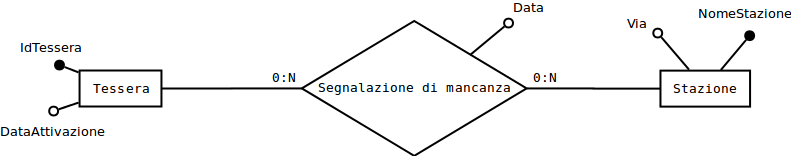
\includegraphics[width=0.5\textwidth]{Immagini-Grafici/Concettuale14.png}
\caption{Modello concettuale}
\end{figure}

\subsection{Vincoli non rappresentati nel modello}
Nel modello concettuale non si riesce a rappresentare tutti i vincoli logici che si sono individuati :
\begin{itemize} %ne ho dimenticati in giro
 \item Un noleggio può essere iniziato (prelevare la bicicletta) solo da una tessera che ha un piano non scaduto.
 \item Un noleggio può essere iniziato (prelevare la bicicletta) solo su una bicicletta in servizio, e lo stato della bicicletta non può venire cambiato finché non viene depositata su una colonnina.
 \item La segnalazione di mancanza riconosce cosa manca (bici o spazi) in base al conteggio delle colonnine che la compongono.
 \item Una segnalazione di rottura di una bicicletta ha come colonnina segnalata una colonnina occupata.
 \item in un trasporto dev'esserci almeno 1 relazione, non è possibile 0.
\end{itemize}
%%%%%%

\section{Progettazione logica}

\section{Implementazione dello schema logico}

\section{Query, procedure, trigger e funzioni}

\section{Interfaccia web}

\end{document}